\section{Introduction}

\begin{frame}
\frametitle{Introduction}
\framesubtitle{Applications}

\begin{figure}
    \begin{minipage}[t]{0.32\linewidth}
        \centering
        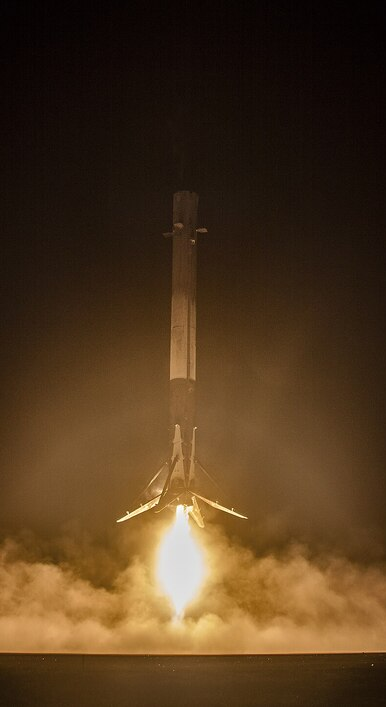
\includegraphics[height=4.5cm]{figures/lanceur_reutilisable.jpg}\\[2pt]
        \parbox{\linewidth}{\centering\scriptsize Lanceur Réutilisable~\cite{spacex}}
    \end{minipage}\hfill
    \begin{minipage}[t]{0.32\linewidth}
        \centering
        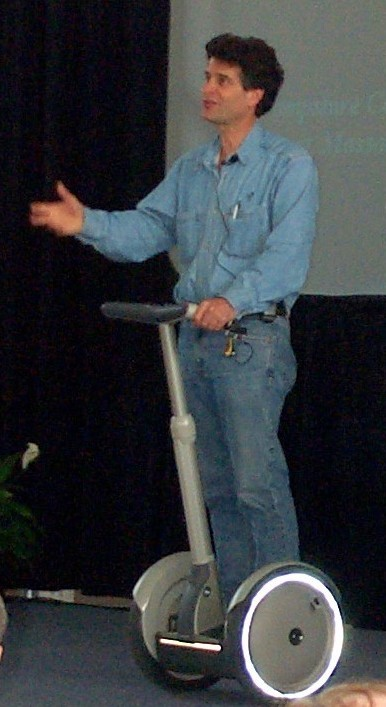
\includegraphics[height=4.5cm]{figures/segway.jpg}\\[2pt]
        \parbox{\linewidth}{\centering\scriptsize Segway~\cite{segway}}
    \end{minipage}\hfill
    \begin{minipage}[t]{0.32\linewidth}
        \centering
        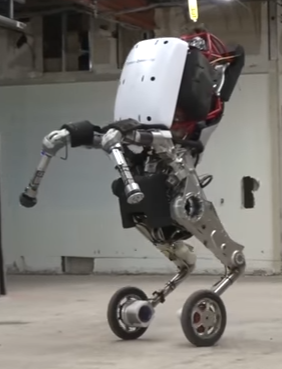
\includegraphics[height=4.5cm]{figures/self_balancing_robot.png}\\[2pt]
        \parbox{\linewidth}{\centering\scriptsize Robot auto-équilibré~\cite{bostondynamics}}
    \end{minipage}
\end{figure}

\end{frame}

%%%%%%%%%%%%%%%%%%%%%%%%%%%%%%%%%%%%%%%%%%%%%%%%

\begin{frame}
\frametitle{Introduction}
\framesubtitle{Le Pendule Inversé}

\begin{figure}
    \begin{minipage}[t]{0.32\linewidth}
        \centering
        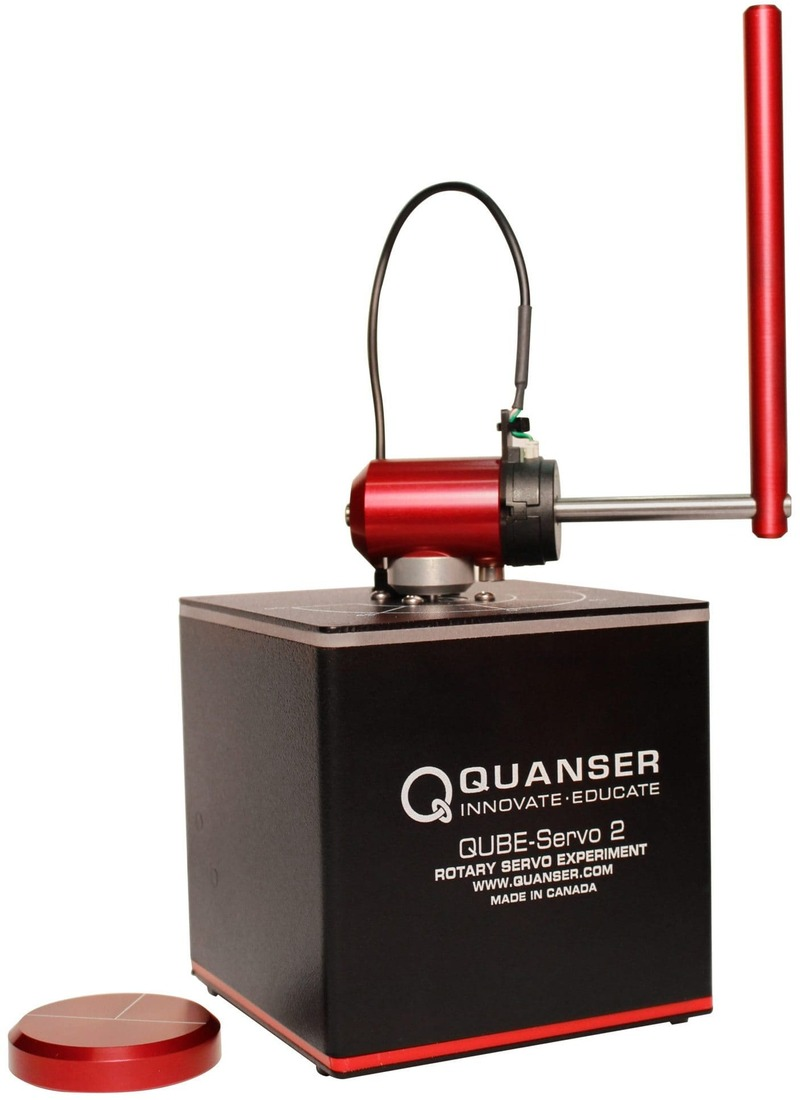
\includegraphics[height=5cm]{figures/inverted_pendulum_rotary.jpg}\\[2pt]
        \parbox{\linewidth}{\centering\scriptsize Pendule inversé rotatif~\cite{quanser_rotary}}
    \end{minipage}\hfill
    \begin{minipage}[t]{0.64\linewidth}
        \centering
        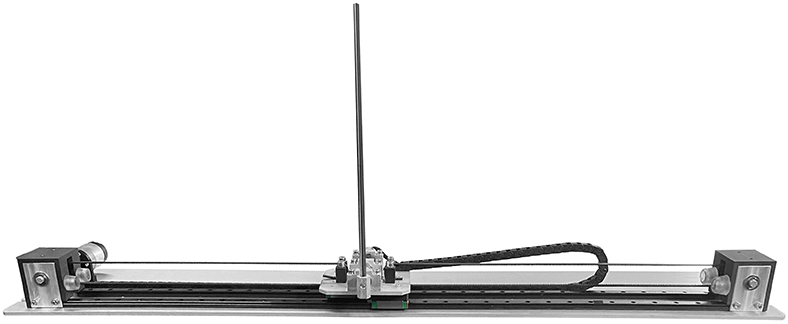
\includegraphics[height=3cm]{figures/inverted_pendulum_linear.png}\\[2pt]
        \parbox{\linewidth}{\centering\scriptsize Pendule inversé sur chariot~\cite{acrome_linear}}
    \end{minipage}
\end{figure}

\end{frame}

%%%%%%%%%%%%%%%%%%%%%%%%%%%%%%%%%%%%%%%%%%%%%%%%

\begin{frame}
\frametitle{Introduction}
\framesubtitle{Problématique}

\vfill
\begin{center}
\begin{tcolorbox}[
    width=0.9\linewidth,
    colback=blue!5,
    colframe=blue!50!black,
    arc=4pt,
    boxrule=1pt,
    fontupper=\large
]
Comment la dynamique d'un système mécanique au voisinage d'un équilibre instable peut-elle être modifiée afin d'assurer sa stabilité au cours du temps, comme dans le cas des lanceurs réutilisables lors de leur retour vertical~?
\end{tcolorbox}
\end{center}
\vfill

\end{frame}

%%%%%%%%%%%%%%%%%%%%%%%%%%%%%%%%%%%%%%%%%%%%%%%%

\begin{frame}
\frametitle{Plan de l'exposé} 
\framesubtitle{Démarche}

\tableofcontents 

\end{frame}
